\documentclass[12pt]{article}
\usepackage{amsmath}
\usepackage{graphicx}
\usepackage{hyperref}
\usepackage[utf8]{inputenc}
\usepackage[T1]{fontenc}
\usepackage[polish]{babel}
%\usepackage{dirtytalk}


\author{Aleksander Głowacki}
\title{Lista nr 2}
\date{05.11.2022}

\begin{document}

\maketitle

\section*{Zadanie 2}

\subsection*{Opis problemu:}
Znajdź DFA o minimalnej liczbie stanów równoważny automatowi

\begin{center} 
    $M = (\{a, b, c, d, e, f, g, h\}, \{0, 1\}, \delta, a, \{d\})$
\end{center}

gdzie $\delta$ ma następującą postać: 

\begin{table}[h]
    %\caption{funkcja przejść}
    \label{epsilon}
    \centering
    \begin{tabular}{c||c|c}
          & \textbf{0} & \textbf{1}\\
        \hline
        \textbf{a} & b & a\\
        \hline
        \textbf{b} & a & c\\
        \hline
        \textbf{c} & d & b\\
        \hline
        \textbf{d} & d & a\\
        \hline
        \textbf{e} & d & f\\
        \hline
        \textbf{f} & g & e\\        
        \hline   
        \textbf{g} & f & g\\
        \hline
        \textbf{h} & g & d\\
    \end{tabular} 
\end{table}

\subsection*{Rozwiązanie:}
\begin{enumerate}
    \item Pierwszym krokiem w redukcji autoamtu jest usunięcie wszystkich stanów, które nie są osiągalne
    ze stanu początkowego.\\
    Z tabeli widzimy, że zbiór wierzchołków, do których możemy przejść ze stanu początkowego
    $a$ ogranicza się do $V' = \{a,b,c,d\}.$
    \\Redukujemy nasz automat $G$ do zbioru wierzchołków $V'$ i zbioru krawędzi z $G$ obciętym do krawędzi między wierzchołkami $\in V'$. Oznaczmy go $G'$.
    \item Rozważamy algorytm redukcji na automacie $G'$ o postaci:\\
    \begin{figure}[htp]
        \centering
        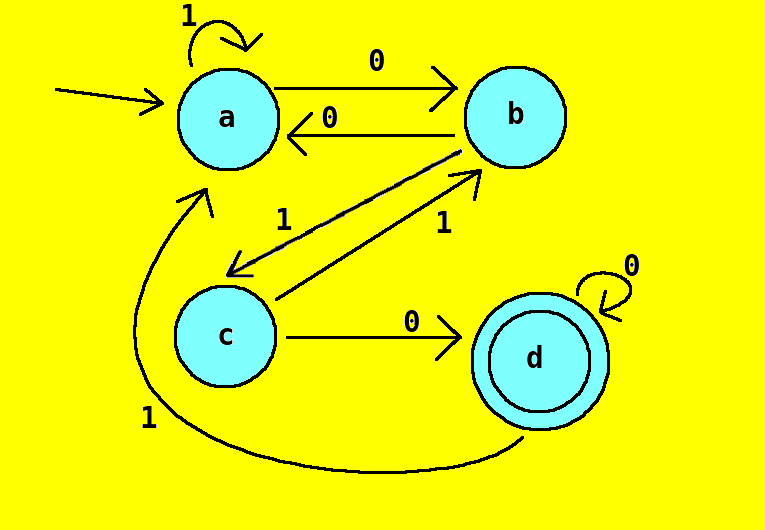
\includegraphics[width=8cm]{automat_kolor.png}
    \end{figure}

    \item Wypełniamy tabelę par stanów, która wskaże pary nierównoważne.\\\\
    "\emph{Dwa stany równoważne to takie,
    że dla każdego x startując z tych stanów albo znajdziemy się 
    równocześnie w stanach akceptujących albo nieakceptujących.}"  $\hspace*{0.2cm}\sim$ wykład 02
    \\Oznaczenia:\\
    $"x"$ - ta para nie jest równoważna\\
    $"$--$"$ - ta komórka w tabeli nie istnieje
    \\Od razu oznaczamy jako nierównoważne pary (stan akceptujący i stan nieakceptujący)
    \begin{table}[h]
        %\caption{funkcja przejść}
        \label{dupa}
        \centering
        \begin{tabular}{c|c|c|c}
            \textbf{b}  & \textbf{c} & \textbf{d} & \\
            \hline
             &  & x & \textbf{a}\\
            \hline
            -- &  & x & \textbf{b}\\
            \hline
            -- & -- & x & \textbf{c}\\
        \end{tabular} 
    \end{table}
    \\Sprawdzamy przejścia par stanów za pomocą $0$ albo $1$.
    
    \begin{itemize}
        \item $(a,b) \xrightarrow[\text{\hspace*{1cm}}]{\text{0}} (b,a)$ - ten przykład jeszcze nic nie mówi
        \item $(a,b) \xrightarrow[\text{\hspace*{1cm}}]{\text{1}} (a,c)$ - sprawdzamy dalej 
        \item $(a,c) \xrightarrow[\text{\hspace*{1cm}}]{\text{0}} (b,d)$ - para stanów nieakceptujących przeszła na parę akcept i nie-akcept.
        \\Zatem stany z par $(a,b)$ i $(a,c)$ nie są równoważne.
        \item $(a,d)$ nierównoważne, bo $a \notin F \land d \in F$
        \item $(c,b) \xrightarrow[\text{\hspace*{1cm}}]{\text{1}} (b,c)$ - pętla, sprawdzamy przejście z $0$
        \item $(c,b) \xrightarrow[\text{\hspace*{1cm}}]{\text{0}} (d,a)$ - nie są równoważne.
    \end{itemize}

    \item  Uzupełnienie tabeli algorytmu:\\\\
    \begin{table}[h]
        %\caption{ostateczna tabela}
        \label{dupa1}
        \centering
        \begin{tabular}{c|c|c|c}
            \textbf{b}  & \textbf{c} & \textbf{d} & \\
            \hline
            x & x & x & \textbf{a}\\
            \hline
            -- & x & x & \textbf{b}\\
            \hline
            -- & -- & x & \textbf{c}\\
        \end{tabular} 
    \end{table}

\end{enumerate}
\newpage
\subsection*{Wnioski:}
    \begin{enumerate}
        \item Automat można obciąć przez usunięcie stanów nieosiągalnych z początkowego.
        \item Później już nie da się go zredukować.
    \end{enumerate}
Ostatecznie DFA minimalny wygląda tak:
\begin{figure}[htp]
    \centering
    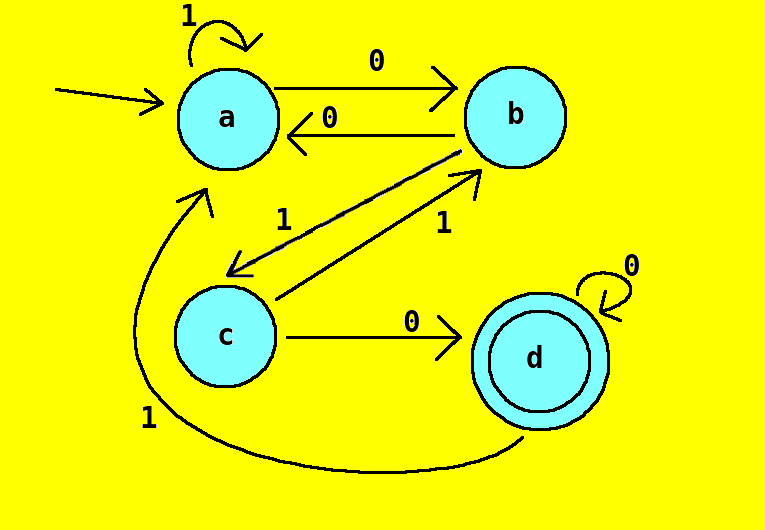
\includegraphics[width=12cm]{automat_kolor.png}
\end{figure}

\end{document}
